%! Author = abenjeddou
%! Date = 29/05/2026


\section{Introduction}
In this chapter, we will present the functional and non-functional needs.
Next, we will identify the use cases in order to create the global case diagram of use as well as the system design.


\section{Requirements specification}

In this section, we will present the objectives of our application, which requires us to identify the actors of the system and the functional needs

\subsection{Actor identification}
This project has one single actor, which is the administrator who manages the entire system. He can preform the following actions:
\begin{itemize}
    \item[-] Manages the Flink Jobs.
    \item[-] Monitors logs and metrics.
\end{itemize}

\subsection{Functional requirements}

Functional requirements or business requirements represent the action that the system must perform, and can only be functional when they are satisfied.
Therefore, our project must mainly cover the following functional needs:
\begin{itemize}
    \item Continuous ingestion of messages from RabbitMQ
    \item Real-time processing of messages.
    \item Transformation and enrichment of messages with information from external services.
    \item Prediction of exceeding data consumption quota using machine learning models.
    \item Dispatching messages once treated.
    \item Implementation of monitoring tools.
\end{itemize}

\subsection{Non-Functional requirements}

In this section, we outline all the non-functional requirements highlighting the constraints to which the system is subject for its operation.

\begin{itemize}
    \item \textbf{High availability:} The system must ensure service continuity by putting
    in place automatic recovery mechanisms in case of failures, thus eliminating
    the single points of failure.
    \item \textbf{Fault tolerance:} The system must be able to handle errors and ensure
    continuity of service by implementing automatic recovery mechanisms
    in case of breakdowns.
    \item \textbf{Scalability:} The system must be able to adapt to the load by increasing
    or reducing resources according to needs, thus ensuring performance
    optimal.
    \item \textbf{Reliability:} The system must offer high performance for the processing of
    real-time data, with minimal latency, thus ensuring a user experience
    quality.
    \item \textbf{Security:} Access to deployment environments and monitoring tools
    must be restricted to authorized users only, thus ensuring data security
    and operations.
\end{itemize}

\section{Use case diagram}

Figure 2.1 represents the global use case diagram, comprised of the following use cases:

\begin{itemize}
    \item \textbf{Manage the Job:}
    This use case encompasses several key actions enabling the administrator to efficiently manage the deployed Flink jobs.
    It includes the following subcases:
    \begin{itemize}
        \item[-] \textbf{Make a Savepoint:}
        The administrator has the ability to trigger the creation of a savepoint for a specific Flink job.
        This allows them to capture the current state of the job and provides a solution for recovery if needed.
        \item[-] \textbf{Stop the Job:}
        This allows the administrator to stop the execution of a running Flink job.
        Stopping the job may be necessary to change the configuration or to resolve potential issues.
        \item[-] \textbf{Configure the Job:}
        The administrator can adjust the Flink job parameters according to specific requirements.
        This includes modifying parallelism, processing configurations, or other essential parameters to optimize performance.
        \item[-] \textbf{Restart the Job:}
        The administrator has the ability to restart a Flink job after making configuration changes or resolving issue.
        Restarting the job ensures that the applied changes are taken into account during execution.
    \end{itemize}

    \item \textbf{Monitor Outputs:}
    \begin{itemize}
        \item[-] \textbf{View Logs and Metrics:}  This involves the continuous monitoring of logs and metrics generated by our system.
        This aims to ensure real-time visibility into the behavior, performance, and potential errors or anomalies.
        \item [-] \textbf{View detected anomalies:} The administrator can view the anomalies detected by the system, which may indicate potential data overconsumption or abnormal behavior.
        This allows for proactive intervention and resolution of problems before they occur.
    \end{itemize}
\end{itemize}

Figure 2.1 below describes the global use case diagram:
\begin{center}
    \centering
    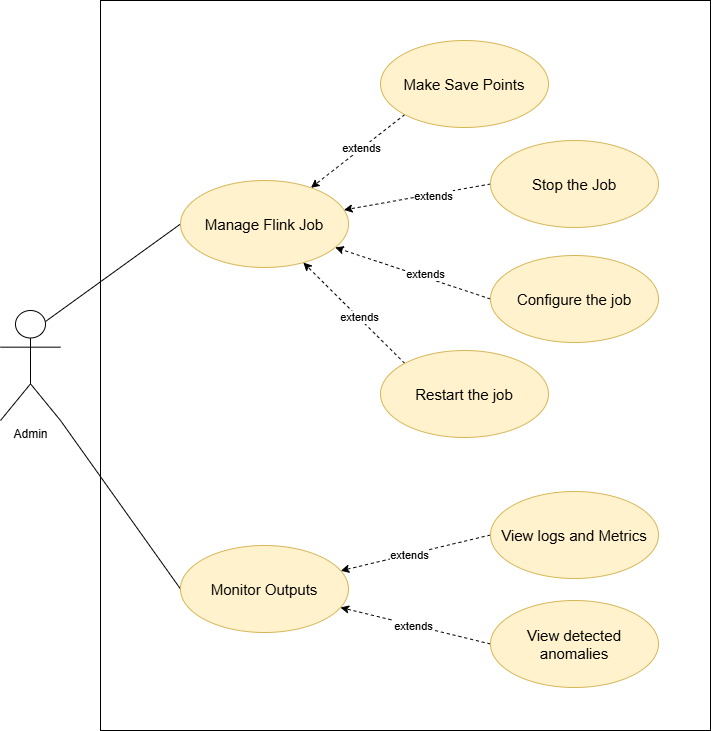
\includegraphics[width=0.9\textwidth,height=9cm]{img/Global Use Case.drawio}
    \captionof{figure}{Global use case diagram}
\end{center}

\section{System design}

\subsection{Sequence diagram of the message processing workflow}

Figure 2.2 details the most important process of our application, encompassing almost all the components implemented in our data stream processing pipeline.
When a message is received in the queue on RabbitMQ, it is consumed by the Flink job and that initiates the processing workflow.
First The message passes through the JSON parser function, where we check the validity of the received message to ensure compatibility with our structure, and we parse it into our \("\)FairUse Message\("\) entity.
Once validated, we retrieve and check the client's subscription to ensure they are eligible for the notification.
If eligible, we proceed to our anomaly detection phase where we run our model on the collected data to predict the chance of data overconsumption.
We add the generated data to our dispatched entity, which is then sent to the DispatcherAPI for delivery to the client.
Finally, after the message is successfully dispatched to the Dispatcher API, we update the client's subscription to keep track of it's latest activity state.

Figure 2.2 shows the sequence diagram of the message processing.
\begin{center}
    \centering
    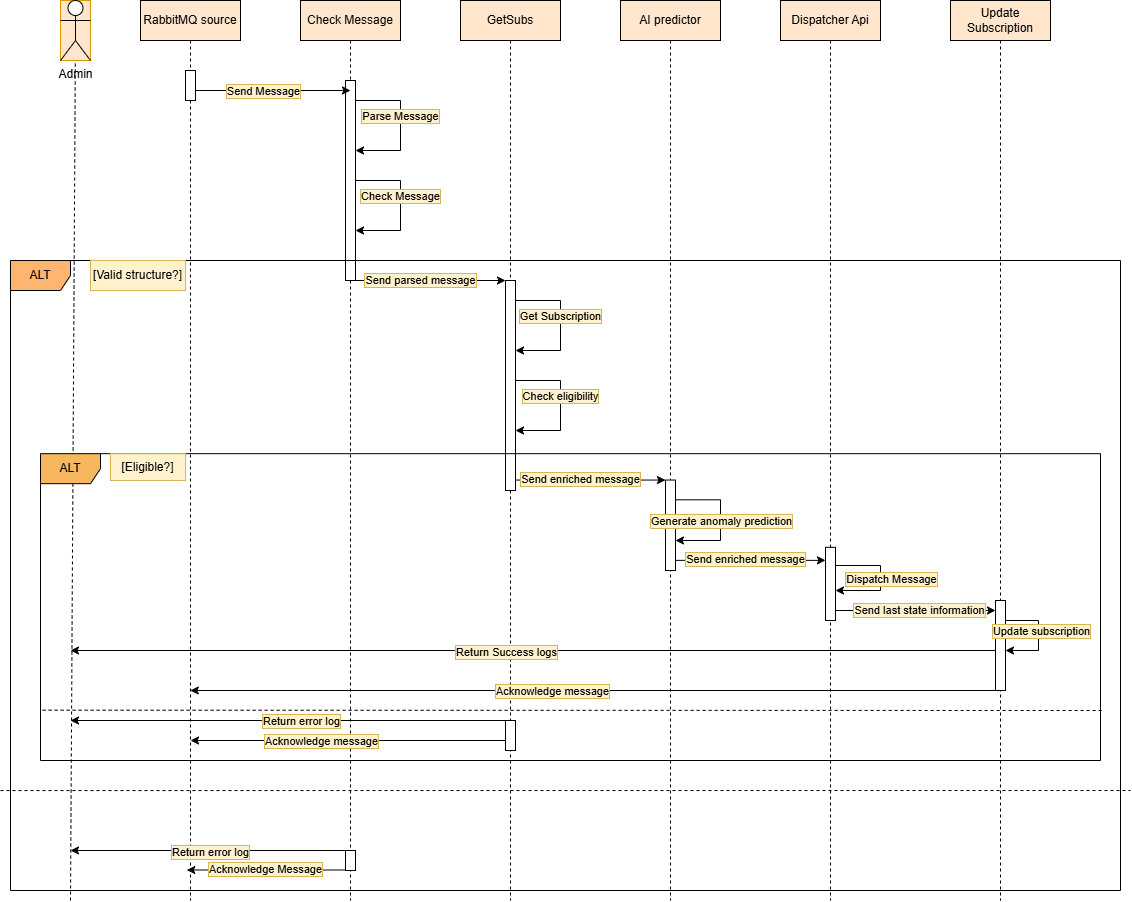
\includegraphics[width=1\textwidth]{img/Diagramme seq}
    \captionof{figure}{Sequence diagram of the message processing workflow}
\end{center}

\subsection{Sequence diagram for subscription retrieval}

Figure 2.3 illustrates the sequence diagram for client subscription retrieval which requires the interaction with external APIs.
We see how the communication is orchestrated by job with the Api gateway and SubsApi.
This interaction is responsible for making sure the system functions with great security and no action is preformed without the correct authentication and authorization.

Initially, the process begins with a call to the tokenServer service to retrieve an OAuth2 authentication token by passing the user and secret as parameters.
This obtained token is then used as a header in the request directed to the API, passing through the ApiGateway beforehand.
The ApiGateway plays a crucial role by validating the token before allowing the request to be transmitted to the external API\@.

Figure 2.3 shows the sequence diagram for subscription retrieval.
\begin{center}
    \centering
    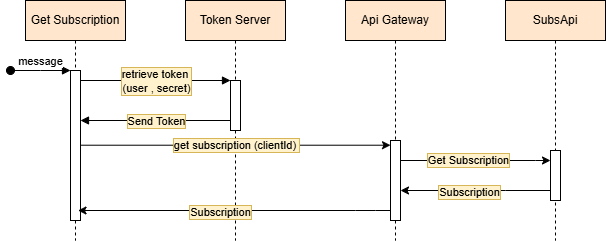
\includegraphics[width=1\textwidth]{img/Diag sec get sub.drawio}
    \captionof{figure}{Sequence diagram for subscription retrieval}
\end{center}

\subsection{Activity diagram}

Figure 2.4 presents the activity diagram describing the process triggered when the Flink job is launched.
The workflow starts by retrieving messages from RabbitMQ, then each message is processed through different stages.
First of, the message, which initially is a String, is converted to a \textbf{FairUse Message}, and we check the validity of its structure.
If the format is invalid, the message is rejected, and processing moves to the next message.
Otherwise, processing continues by retrieving the client subscription.
The system then checks if the client is eligible for the notification.
If the client is not eligible, the message is discarded.
Otherwise, the next step consists of sending passing the data collected to the anomaly detection model, which predicts the chance of data overconsumption and adds it to our message.
Finally, the message is sent to the DispatcherAPI that handles notification delivery to the client, and the subscription is updated to reflect the latest state.

Figure 2.4 shows the activity diagram of the message processing workflow.
\begin{center}
    \centering
    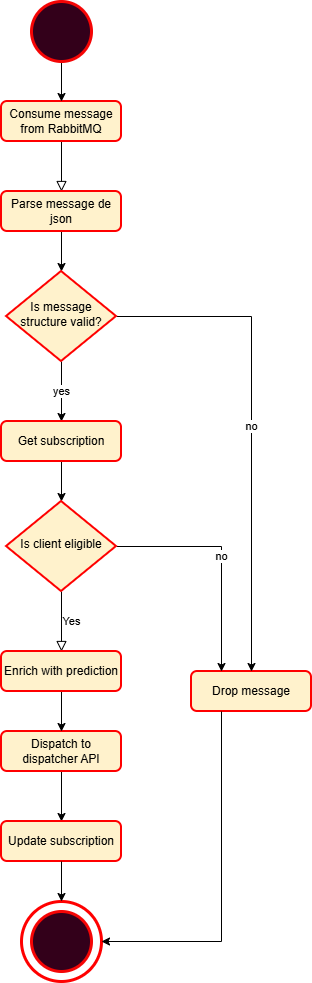
\includegraphics[width=0.6\textwidth, height=17cm]{img/Diag activity.drawio}
    \captionof{figure}{Activity diagram}
\end{center}

\section*{Conclusion}
In this chapter, we started by analyzing the functional and non-functional requirements of our system.
Then in second section we showcased the various use cases involving the system's actor with a use case diagram.
Finally, we explained the design of our application using sequence diagrams for the main steps of our solution, accompanied by an activity diagram.
This step allows us to present the detailed architecture of our solution in the next chapter.
